\documentclass[10pt]{article}

% RLJ/RLC 2026 submission mode. Use [accepted] or [preprint] only for those
% versions of the paper.
\usepackage[preprint]{rlj}

\usepackage{amssymb}
\usepackage{array}
\usepackage{float}
\usepackage{graphicx}
\usepackage{placeins}
\usepackage{tikz}
\usepackage{xurl}

\graphicspath{{figures/}}

\newcommand{\papergrid}[2][0.18]{%
  \begin{tikzpicture}[x=#1cm,y=-#1cm,baseline=(current bounding box.center)]
    \fill[white] (0,0) rectangle (10,10);
    #2
    \draw[step=1,gray!35,line width=0.18pt] (0,0) grid (10,10);
    \draw[gray!55,line width=0.35pt] (0,0) rectangle (10,10);
  \end{tikzpicture}%
}

\newcommand{\papervertical}{%
  \foreach \r in {0,...,9}{\fill[black] (5,\r) rectangle +(1,1);}%
}

\newcommand{\paperdiagonal}{%
  \foreach \i in {0,...,9}{\fill[black] (\i,\i) rectangle +(1,1);}%
}

\newcommand{\papersquare}{%
  \foreach \i in {0,...,9}{%
    \fill[black] (\i,0) rectangle +(1,1);
    \fill[black] (\i,9) rectangle +(1,1);
    \fill[black] (0,\i) rectangle +(1,1);
    \fill[black] (9,\i) rectangle +(1,1);%
  }%
}

\newcommand{\papergridlabel}[3][0.18]{%
  \begin{tabular}{@{}c@{}}
    \papergrid[#1]{#2}\\[-0.15em]
    {\scriptsize #3}
  \end{tabular}%
}

\title{On the Value of Abstractions: Abstraction Selection in Bounded Program Synthesis}
\setrunningtitle{Abstraction Selection in Bounded Program Synthesis}
\hypersetup{
  pdftitle={On the Value of Abstractions: Abstraction Selection in Bounded Program Synthesis},
  pdfauthor={Adam Cuculich}
}

\author{Adam Cuculich}
\emails{adam@cuculich.me}
\affiliations{}

\keywords{abstraction selection, bounded program synthesis, library learning, search utility}

\summary{Reusable abstractions can shorten programs in program synthesis. Some
do not improve bounded search. We compare two selection procedures on a
synthetic grid benchmark.
With ten abstractions, both procedures solved more problems than primitive-only
search. Utility solved 4.08 more test problems per 100 than
compression on acquired validation solutions (95 percent CI 2.46 to 5.71).
This comparison includes the objective and solution availability. At 30,000
attempts, observed mean performance was highest at 11 abstractions. With 20
abstractions, both procedures performed worse than primitives. In this
benchmark, abstraction value depended on selection method, library size, and
search budget.}

\contribution{
Validation Search Utility selects the abstractions that decrease capped search
cost most on separate validation targets.
}{
Compression selects the abstractions that shorten known solutions most.
}

\contribution{
With ten abstractions, both procedures solved more test problems than
primitive-only search. Utility solved 4.08 more test problems per 100 than
compression on acquired validation solutions.
}{
Starter problems provide the same candidate set for both procedures. Separate test
problems measure held-out performance.
}

\contribution{
At 30,000 attempts, observed mean performance was highest at 11 abstractions.
With 20 abstractions, both procedures performed worse than primitives alone.
}{
For these fixed one- and two-abstraction libraries, a larger budget reversed
the decrease.
}

\begin{document}

\maketitle

\begin{abstract}
Reusable abstractions can shorten programs in program synthesis. However, each
item also expands the solver's search space. With a fixed budget, this added
search can prevent the solver from reaching a shorter solution. We ask when
abstraction libraries improve bounded synthesis and what determines their
value. The answer matters because future savings must justify selection and
added search costs.
To test this question, we compare two abstraction-selection procedures in
Pattern Builder, a synthetic grid benchmark with deterministic, size-ordered
search. Across 30 random problem worlds, both procedures select from the same
starter-derived candidate set. Compression selects candidates that shorten
acquired solutions. Validation Search Utility selects candidates that reduce
capped search cost on separate validation targets. We evaluate each selected
library on the same held-out test problems. We then vary library size and search
budget.
With ten abstractions, both procedures outperformed search with the original
domain-specific language (DSL), which contained no added abstractions. Utility
solved 4.08 more test problems per 100 than validation-solution compression (95
percent CI 2.46 to 5.71). This comparison includes the scoring rule and
compression's available solutions. Utility's advantage over standard
compression, based on 100 starter problems, remained uncertain. At 30,000
attempts, mean performance peaked near 11 abstractions and fell below the
original DSL at 20. For both procedures, performance also decreased when the
library grew from one abstraction to two. To test whether the budget caused
this decrease, we held those libraries fixed and increased only the budget. The
decrease reversed. This result supports a search-cutoff explanation: added
abstractions can consume the budget before the solver reaches larger programs
where they help. Utility also required more search during selection, and some
cases did not recover that cost. Therefore, solution compression alone does not
measure an abstraction's value under bounded search. A library should be
evaluated with its intended solver, budget, workload, and expected reuse.
\end{abstract}

\section{Introduction}

Reusable abstractions can accelerate program synthesis. They can replace
several operations with one library item. However, each abstraction also
increases the set of programs that a solver can construct. With a fixed search
budget, the number and content of the abstractions can determine whether the
solver finds a solution. This paper asks which abstractions to keep, how many
to keep, and when the search budget prevents a useful library from helping.
We study these questions in Pattern~Builder. The solver must reproduce a binary
$10\times10$ target grid without an input grid. It combines six primitive grids
with fixed unary and binary operators until an expression matches the target.
Figure~\ref{fig:problem-solution} shows one solution. It uses \texttt{add}, which
returns the union of two grids.
\begin{figure}[H]
  \centering
  \begin{tabular}{@{}c@{\hspace{0.03\linewidth}}c@{}}
    \parbox{0.25\linewidth}{\centering\textbf{Target}}
    &
    \parbox{0.70\linewidth}{\centering\textbf{One valid solution}}
    \\[0.5em]
    \begin{minipage}[t]{0.25\linewidth}
      \vspace{0pt}
      \centering
      \papergridlabel[0.20]{\papersquare\papervertical\paperdiagonal}{target grid}
    \end{minipage}
    &
    \begin{minipage}[t]{0.70\linewidth}
      \vspace{0pt}
      \centering
      \papergridlabel[0.125]{\papervertical}{\texttt{line\_vertical}}
      \hspace{0.25em}$+$\hspace{0.25em}
      \papergridlabel[0.125]{\papersquare}{\texttt{square}}
      \hspace{0.25em}$+$\hspace{0.25em}
      \papergridlabel[0.125]{\paperdiagonal}{\texttt{diagonal}}
      \hspace{0.25em}$=$\hspace{0.25em}
      \papergridlabel[0.125]{\papersquare\papervertical\paperdiagonal}{output}
      \\[0.7em]
      \texttt{add(add(line\_vertical, square), diagonal)}
    \end{minipage}
  \end{tabular}
  \caption{A grid target and one expression that reproduces it.}
  \label{fig:problem-solution}
\end{figure}
The solver can store an intermediate grid as a library item. We call this
stored grid an \emph{abstraction}. In Figure~\ref{fig:problem-solution}, the
solver could store the union of the vertical line and the square. This would
reduce the solution from two operations to one. The abstraction is a fixed
grid, not a learned operator. We change the library and keep the operators
fixed.
An abstraction can shorten a solution, but it also becomes an available
argument for the operators. This creates more small programs. The solver
examines all smaller programs first. These programs can use the budget before
the solver reaches a larger program where the abstraction helps. Therefore,
\[
  \text{shorter known solutions}
  \not\Rightarrow
  \text{less search on unseen problems}.
\]
Compression selects abstractions that remove the most operations from known
solutions. It measures the shortcut benefit. Its score excludes the extra search
that the larger library creates. Validation search utility selects abstractions by their
effect on bounded search for separate validation targets. All procedures use
the same candidate menu, which comes from starter problems. Validation data can
change which candidates are selected, but cannot add candidates. Test data only
evaluate the selected libraries on unseen targets.
Both validation procedures use the same 25 problems. Utility scores all search
outcomes, including failures. Validation-solution compression scores acquired
solution programs and omits unsolved problems. Thus, the procedures use
different evidence.
\textbf{Experiment I} compares the procedures and tests the effect of similarity
between the starter and test problem sets.
\textbf{Experiment II} varies library size. \textbf{Experiment III} varies the
search budget while the libraries stay fixed. Together, they test selection
method, library size, and search budget.
\section{Related Work}

Library learning adds reusable program components to make later synthesis
easier. Many systems select these components by compressing known solution
programs. DreamCoder learns a function library together with a neural search
policy \citep{ellis2021dreamcoder}. Stitch finds functions that minimize the cost
of a rewritten program corpus \citep{bowers2023stitch}. A recent study used
Pattern Builder to examine human helper choices under changing task structure
\citep{hernandezcano2026prospective}. Human choices were consistent with
compression of expected future solutions. Our study instead measures how
automated abstraction selection changes bounded search.

Iba described the underlying search tradeoff. Macros shorten solution paths and
increase the search branching factor \citep{iba1989macro}. AbstractBeam later
added Stitch abstractions to guided bottom-up synthesis
\citep{zenkner2024abstractbeam}. It improved performance on related tasks. A
distribution shift removed this benefit, and unused abstractions could enlarge
the language. AMaze provides a close technical comparison. It modifies a DSL
using predicted synthesis time. AMaze predicts this time from the enumeration
rank of solver-specific program fragments. Its whole-program compression
baseline slowed two of four synthesizers \citep{ye2026amaze}. Our work measures capped
cost directly with exact enumeration over a fixed menu within each seed. It
varies library size and changes only the budget for fixed libraries. It also
measures the work used to select each library. These controls test how selection
method, library size, and budget jointly determine abstraction value.
\section{Methodology}

\subsection{Experiment Overview}

We test how abstraction selection affects bounded-search performance. Later
experiments change library size and search budget. Experiment I compares four
selection procedures. Each procedure selects from the same candidate menu. We
then test each selected library on held-out problems.
Starter problems create the candidate menu and supply solutions for
starter-based compression. The validation-based procedures use separate
validation problems. We reserve the test problems for held-out evaluation.
We repeat the experiment across 30 random problem worlds. A seed creates one
world with 12 hidden motifs and one starter set. Six primary conditions share
that world. Each condition has separate validation and test problems.
Table~\ref{tab:problem-sets} gives the size and purpose of each problem set.

\begin{table}[H]
  \centering
  \small
  \caption{Problem sets and their use.}
  \label{tab:problem-sets}
  \vspace{0.7em}
  \begin{tabular*}{0.95\linewidth}{@{\extracolsep{\fill}}p{0.21\linewidth}rp{0.64\linewidth}@{}}
    \hline
    \textbf{Problem Set} & \textbf{Size} & \textbf{Purpose} \\
    \hline
    \noalign{\vskip 0.25em}
    Starter Problems & 100 & Creates the candidate menu and supplies problems for starter-based compression. \\
    Validation Problems & 25 & Guides validation-solution compression and validation utility. \\
    Test Problems & 100 & Measures each selected library on held-out problems. \\
    \hline
  \end{tabular*}
\end{table}

Each seed has one menu of 50 candidate abstractions. Every selection procedure
within that seed uses this menu. Solutions to starter problems create the menu. Validation
evidence changes which candidates a procedure selects. Test problems only
measure the selected libraries.
Table~\ref{tab:selection-procedures} defines the four selection procedures.

\begin{table}[H]
  \centering
  \footnotesize
  \caption{Four selection procedures in Experiment I.}
  \label{tab:selection-procedures}
  \vspace{0.7em}
  \setlength{\tabcolsep}{4pt}
  \renewcommand{\arraystretch}{1.12}
  \begin{tabular*}{0.95\linewidth}{@{\extracolsep{\fill}}>{\raggedright\arraybackslash}p{0.07\linewidth}>{\raggedright\arraybackslash}p{0.21\linewidth}>{\raggedright\arraybackslash}p{0.14\linewidth}>{\raggedright\arraybackslash}p{0.23\linewidth}>{\raggedright\arraybackslash}p{0.218\linewidth}@{}}
    \hline
    \textbf{ID} & \textbf{Procedure} & \textbf{Problems} & \textbf{Search during selection} & \textbf{Score} \\
    \hline
    \noalign{\vskip 0.25em}
    \mbox{$S_{100}$} & Standard compression & 100 starter & Acquire solutions; 30,000 attempts per problem & Remaining operations in acquired solutions \\
    \mbox{$S_{25}$} & Starter-subset compression & 25 starter & Acquire solutions; 30,000 attempts per problem & Remaining operations in acquired solutions \\
    \mbox{$M$} & Validation-solution compression & 25 validation & Acquire solutions; 90,000 attempts per problem & Remaining operations in acquired solutions \\
    \mbox{$U$} & Validation utility & 25 validation & Score each trial library; 30,000 attempts & Mean capped search cost for all 25 targets \\
    \hline
  \end{tabular*}
\end{table}

Each compression procedure runs a separate target-directed search for each
scoring problem. It keeps the first solution found and omits unsolved problems.
Utility runs one size-ordered search for each trial library. The resulting
output record scores all 25 validation targets. An unreached target receives
the maximum cost of 30,000. Hidden generator programs are never selector
inputs. A fixed seeded shuffle selects the 25 starter problems for $S_{25}$.
All six conditions within a seed use the same subset. Across the 180 primary
Experiment I cells, $S_{100}$ acquired solutions for a mean of 62.70 of 100 problems.
$S_{25}$ acquired solutions for 16.33 of 25, and $M$ acquired solutions for
16.59 of 25.

In Experiment I, each procedure selects ten abstractions. We evaluate every
selected library on the same 100 test problems with a 30,000-attempt limit.
The primary comparison starts with the same 25 validation problem identities.
Utility scores all 25 target outcomes. Validation-solution compression scores
only acquired solution programs and omits a mean of 8.41 unsolved problems.
The comparison holds the candidate menu, test problems, library size, and test
budget constant. It includes the scoring objective and the usable evidence.
Thus, it compares complete procedures.

\subsection{Synthesis and Bounded Search}

Each problem supplies one binary target grid $T$. The primitive-only library
$L_0$ contains six grids: blank, horizontal line, vertical line, diagonal,
square, and triangle. The current ordered library is $L$. A program is a
library item or an operator applied to one or two programs. The unary operators
are invert, a left-to-right flip, a top-to-bottom flip, and diagonal
reflection. The diagonal runs from the upper-left corner to the lower-right
corner. Invert changes each black cell to white and each white cell to black.
The binary operators are \texttt{add} (union), \texttt{subtract} (set
difference), and \texttt{overlap} (intersection). Program $P$ produces grid
$\operatorname{eval}(P)$. It solves $T$ when $\operatorname{eval}(P)=T$.
Program size is the number of operator applications. A primitive or stored
abstraction has size zero. Let $B$ be the maximum number of candidate programs
that the solver can try. The deterministic bottom-up solver tries programs in
order of increasing size. It stops after $B$ attempts or after it has tried all
programs with seven or fewer operator applications. The solver keeps the first
program for each distinct output grid. The implementation fixes the order of
operators, child-program sizes, and commutative arguments. Each complete program
counts as one attempt. This count includes a duplicate that the solver later
discards.
For utility scoring and final evaluation, one size-ordered search records all
outputs for a library. This record gives the first attempt that produced each
target. Compression uses separate target-directed searches to acquire solution
programs.
For target $T$ and library $L$, the capped search cost is
\begin{equation}
  N_B(T,L)=
  \begin{cases}
    n, & \text{if target $T$ first appears at attempt $n\leq B$},\\
    B, & \text{if the solver does not reach $T$ within the budget}.
  \end{cases}
\end{equation}
Unless stated otherwise, $B=30{,}000$. The primary outcome is the number of
the 100 held-out test targets that the solver reaches.

\subsection{The Abstraction Candidate Menu}

An abstraction stores a reached grid as a size-zero library item. For each
seed, the primitive-only solver tries 30,000 programs and records distinct
grids. It runs to the budget. We keep nonblank, nonprimitive grids whose first
program has one to four operations. A grid supports a starter target when one
invert or reflection produces that target. It also supports the target when
one add or subtract with another reached grid produces it. We keep grids that
support at least two starter targets. We rank candidates by decreasing support
count. We break ties by the attempt at which the solver first reached the grid,
then by program string. The top 50 form the candidate menu $\mathcal C$, from which
abstractions are later selected. Abstraction candidate discovery does not use validation or test data.

\subsection{Selection Procedures}

Let $K$ be the number of abstractions to select. We run each selection
procedure separately. For one run, let $A_0=()$. After $k$
selections, $A_k=(a_1,\ldots,a_k)$ is the ordered list of selected
abstractions. Library $L(A_k)$ contains the primitives followed by this list.
The order matters because it changes the solver's search order. The notation
$A\mathbin{\|}a$ means list $A$ followed by abstraction $a$. For cost function
$J$, the greedy selection procedure is
\begin{equation}
  \begin{aligned}
    a_k
      &=\arg\min_{\substack{a\in\mathcal C\\a\notin A_{k-1}}}
          J\!\left(A_{k-1}\mathbin{\|}a\right),\\
    A_k
      &=A_{k-1}\mathbin{\|}a_k,
        \qquad k=1,\ldots,K.
  \end{aligned}
\end{equation}
Compression and utility use different costs and tie rules. Compression scores
acquired solution programs. Let $\mathcal P_{\mathrm{sol}}$ contain the first
solution found for each solved scoring problem. For program $P$, let
$\operatorname{children}(P)$ be its ordered list of immediate child programs.
For selected abstraction list $A$, the number of remaining operations is
\begin{equation}
  n_{\mathrm{ops}}(P,A)
  =
  \begin{cases}
    0,
      & \text{if }\operatorname{children}(P)=()
        \text{ or }\operatorname{eval}(P)\in A,\\
    1+\displaystyle\sum_{P'\in\operatorname{children}(P)}
        n_{\mathrm{ops}}(P',A),
      & \text{otherwise}.
  \end{cases}
\end{equation}
A subtree whose output is in $A$ becomes one size-zero library item. Its
internal operations contribute zero. Let $\mathcal T_{\mathrm{util}}$ contain
the targets used to score utility. The two costs are
\begin{equation}
  \begin{aligned}
    J_{\mathrm{comp}}(A)
      &=\sum_{P\in\mathcal P_{\mathrm{sol}}}n_{\mathrm{ops}}(P,A),\\
    J_{\mathrm{util}}(A)
      &=\frac{1}{|\mathcal T_{\mathrm{util}}|}
        \sum_{T\in\mathcal T_{\mathrm{util}}}N_B\!\left(T,L(A)\right).
  \end{aligned}
\end{equation}
Compression sets $J=J_{\mathrm{comp}}$. Utility sets
$J=J_{\mathrm{util}}$. Utility assigns cost $B$ to any target the solver does
not reach within $B$ attempts. Thus, when $B=30{,}000$, an unreached target has
cost $30{,}000$. If two candidates have the same compression cost, Compression
compares their text forms in lexicographic order. This rule compares characters
from left to right. For example, \texttt{add(diagonal, square)} comes before
\texttt{add(line\_vertical, square)} because \texttt{d} comes before \texttt{l}.
If two trial libraries have the same utility cost, Utility first selects the
library that solves more targets. If both libraries solve the same number,
Utility applies the same text-order rule.

\subsection{Problem Sets and Problem-Set Similarity}

Each seed defines 12 hidden motifs, with four each at two, three, and four
operations. From these motifs, the generator creates 100 starter, 25 validation,
and 100 test problems. Each problem uses two or three distinct motifs combined
from left to right with uniformly sampled binary operators and up to two unary
operators. Fixed schedules set the motif and unary-operator counts. The
generator rejects invalid and duplicate grids. Selection procedures receive
only target grids or acquired solutions. They do not receive motif identities
or hidden programs.
Starter problems use motif probabilities $\mathbf p_{\mathrm{start}}$. We
define $\mathbf p_{\mathrm{alt}}$ by reversal or random permutation. Reversal
changes $(p_1,\ldots,p_{12})$ to $(p_{12},\ldots,p_1)$. Common starter motifs
then become rare, and rare starter motifs become common. A random permutation
assigns the same probability values to different motifs. The shift parameter
$\alpha\in\{0,0.5,1\}$ sets the future probabilities:
\[
  \mathbf p(\alpha)
    =(1-\alpha)\mathbf p_{\mathrm{start}}
      +\alpha\mathbf p_{\mathrm{alt}}.
\]
The values $\alpha=0$, $0.5$, and $1$ use the starter probabilities, an equal
mixture, and the alternative probabilities. In each primary condition,
validation and test problems are separate draws from $\mathbf p(\alpha)$.
Combining two alternatives with three values of $\alpha$ gives six conditions
per seed. The two conditions at $\alpha=0$ use separate target draws. We
measure realized problem-set similarity, $\rho$, between the starter and test
sets. It is the Spearman correlation between their motif-count vectors. We use
$\rho$ only for analysis. It requires hidden motif identities and the completed
test set.

\subsection{Experiments}

Let $m$ identify a selection method, $i\in\{1,\ldots,30\}$ a seed, and
$c\in\{1,\ldots,6\}$ a problem-set similarity condition. Outcome
$Y_{ic}^{m}(K,B)$ is the number of test problems that method $m$ solves with
budget $B$ and its first $K$ abstractions. Thus,
$Y_{ic}^{m}(K,B)\in\{0,\ldots,100\}$. The seed mean and
experiment mean are
\begin{equation}
  \bar Y_i^{m}(K,B)=\frac{1}{6}\sum_{c=1}^{6}Y_{ic}^{m}(K,B),
  \qquad
  \widehat\mu^{m}(K,B)=\frac{1}{30}\sum_{i=1}^{30}\bar Y_i^{m}(K,B).
\end{equation}
Each seed gives six related outcomes. We average them into one seed score, then
average the 30 scores. Because each seed has six conditions, the experiment
mean equals the mean of all 180 cells. Conditions have equal weight. Only the
30 seeds are independent.

\paragraph{Experiment I: Which Abstractions?}
Experiment I compares the four procedures. It also tests whether problem-set
similarity changes the difference between utility and standard compression.
Thirty seeds under six primary conditions gave 180 cells. The 30 registered
stale-validation cells used validation problems at $\alpha=0.5$ and test
problems at $\alpha=1$. They formed a separate stress test of outdated
validation data. We excluded them from the primary estimates because those
estimates require validation and test problems from the same distribution.
Each primary cell used $K=10$, one candidate menu, and the same held-out test
targets for all procedures.
Table~\ref{tab:selection-procedures} defines $U$, $M$, $S_{25}$, and $S_{100}$.
Standard compression, $S_{100}$, is the practical comparator. Post hoc, utility
also scored the same 25 starter problems as $S_{25}$. Using the experiment mean
$\widehat\mu^{m}(K,B)$ defined above, the registered contrasts are
\begin{equation}
  \begin{aligned}
    C_{U-M}
      &=\widehat\mu^{U}(10,30{,}000)
        -\widehat\mu^{M}(10,30{,}000),\\
    C_{M-S_{25}}
      &=\widehat\mu^{M}(10,30{,}000)
        -\widehat\mu^{S_{25}}(10,30{,}000).
  \end{aligned}
\end{equation}
A positive value favors the first procedure in each subscript. Contrast
$C_{U-M}$ compares the complete validation procedures. Contrast $C_{M-S_{25}}$
compares two complete compression procedures. They differ in scoring-problem
source and acquisition budget.
Let $W_m$ count the candidate-program attempts used to select procedure $m$'s
library. Utility scores 455 trial libraries with at most 30,000 attempts each.
The work $W_M$ includes validation-solution acquisition. The work $W_{S_{100}}$
treats prior starter-solution acquisition as a sunk cost. These counts exclude
compression segmentation.
Let $\bar N_m$ be the mean capped cost across the 100 held-out test problems.
For comparator $m\in\{M,S_{100}\}$, $n_{\mathrm{pay}}(m)$ is the number of
future problems needed to recover utility's additional selection work:
\begin{equation}
  n_{\mathrm{pay}}(m)
  =
  \begin{cases}
    \left\lceil
      \dfrac{\max(0,W_U-W_m)}
            {\bar N_m-\bar N_U}
    \right\rceil,
      & \text{if } \bar N_m>\bar N_U,\\
    \infty,
      & \text{if } \bar N_m\leq\bar N_U.
  \end{cases}
\end{equation}
This post hoc calculation assumes constant mean savings and uses only program
attempts. We hypothesized that starter-based compression would improve relative
to $U$ as starter and test motif frequencies became more similar. Repeated
motifs can let starter abstractions help test problems. For assigned shift, we
averaged the two alternative assignments. We then calculated each procedure
difference at $\alpha=1$ minus $\alpha=0$.
Regressions related these differences to realized problem-set similarity $\rho$
with seed fixed effects and seed-clustered standard errors.

\paragraph{Experiment II: Library Size.}
Thirty fresh seeds (6541--6570) and six conditions formed 180 cells. Standard
compression, validation-solution compression, and utility each selected one
ordered sequence of 20 abstractions. We evaluated every prefix from $K=0$ to
$K=20$ with $B=30{,}000$. The value $K=0$ is the primitive-only library.
Selection ran once for each sequence.
For methods $m$ and $m'$, set $B=30{,}000$. Their performance difference at
library size $K$ is
\begin{equation}
  D_{m,m'}(K)
    =\widehat\mu^{m}(K,B)-\widehat\mu^{m'}(K,B).
\end{equation}
The registered method contrasts were $D_{U,M}(20)$,
$D_{U,S_{100}}(20)$, and the change in $D_{U,M}$ from $K=10$ to $K=20$.
Two registered within-procedure contrasts measured the changes in
$\widehat\mu^U$ and $\widehat\mu^{S_{100}}$ from $K=10$ to $K=20$.
Observed peaks and the one-to-two drop were descriptive.

\paragraph{Experiment III: Search Budget.}
Experiment III reused Experiment II's exact $K=1$ and $K=2$ libraries. It varied
only $B\in\{30{,}000,45{,}000,60{,}000,90{,}000\}$. Worlds, targets,
abstraction order, size limit, and enumeration order remained fixed. Here, $m$
identifies the fixed library selected in Experiment II. Selection did not run
again. For $m\in\{S_{100},U\}$, the effect of the second abstraction is
$\Delta_m(B)$. The budget interaction is $I_m$:
\begin{equation}
  \begin{aligned}
    \Delta_m(B)
      &=\widehat\mu^m(2,B)-\widehat\mu^m(1,B),\\
    I_m
      &=\Delta_m(90{,}000)-\Delta_m(30{,}000).
  \end{aligned}
\end{equation}
A positive $I_m$ means that increasing the search budget raises the $K=2$ minus
$K=1$ performance difference. We calibrated the budgets on ten previously
analyzed sensitivity seeds before we inspected above-30,000 outcomes for the
Experiment II seeds.

\subsection{Statistical Analysis}

Primary comparisons average six related differences between procedures into
one seed-level difference. The 30 seed-level differences test whether the
advantage repeats across worlds. Similarity analyses keep conditions separate
because similarity varies by condition. They treat conditions that share a
seed as related. The two primary comparisons use two-sided 95\% confidence
intervals based on Student's $t$ distribution.
Each interval uses the mean and variation of the 30 differences. The $t$
distribution accounts for
uncertainty in the estimated variation. The capacity study tracks method differences across
$K=1,\ldots,20$. The budget study tests whether more search changes the
one-to-two abstraction loss. Both use maximum-$t$ intervals from 10,000
seed-level bootstrap resamples for related estimates. Experiment I registered
its contrasts and directions before data collection, but selected the
Student-$t$ interval afterward. The capacity analysis preceded fresh data. Its
results motivated the registered budget hypothesis and budget increase. Later
analyses are descriptive or post hoc.

\section{Results}

\subsection{Experiment I: Which Abstractions?}

With ten abstractions, validation utility solved 66.08 test problems
(Figure~\ref{fig:study1-selection}). Validation-solution compression acquired
solutions for a mean of 16.59 of the 25 validation problems and omitted 33.6\%.
It solved 62.00 test problems. The difference was 4.08 (95\% CI [2.46, 5.71]).
Both used one menu and validation set. Utility scored all outcomes, including
failures. Compression scored acquired programs and omitted the rest. Thus, the
difference includes the scoring objective and
solution availability.
The primitive-only library solved 58.91 problems. Standard compression, which
used all 100 starter problems, solved 64.53. Validation-solution compression solved 0.26
fewer problems than compression on the 25-problem starter subset (95\% CI
[$-1.46$, 0.95]). Utility's 1.55-problem advantage over standard compression
remained uncertain because its 95\% CI [$-0.27$, 3.37] included zero. Utility
outperformed validation-solution compression. In the separate
stale-validation stress test, utility solved a mean of 65.60 test problems.
Validation-solution compression solved 61.00, and standard compression solved
65.40.
\FloatBarrier
\begin{figure}[!htbp]
  \centering
  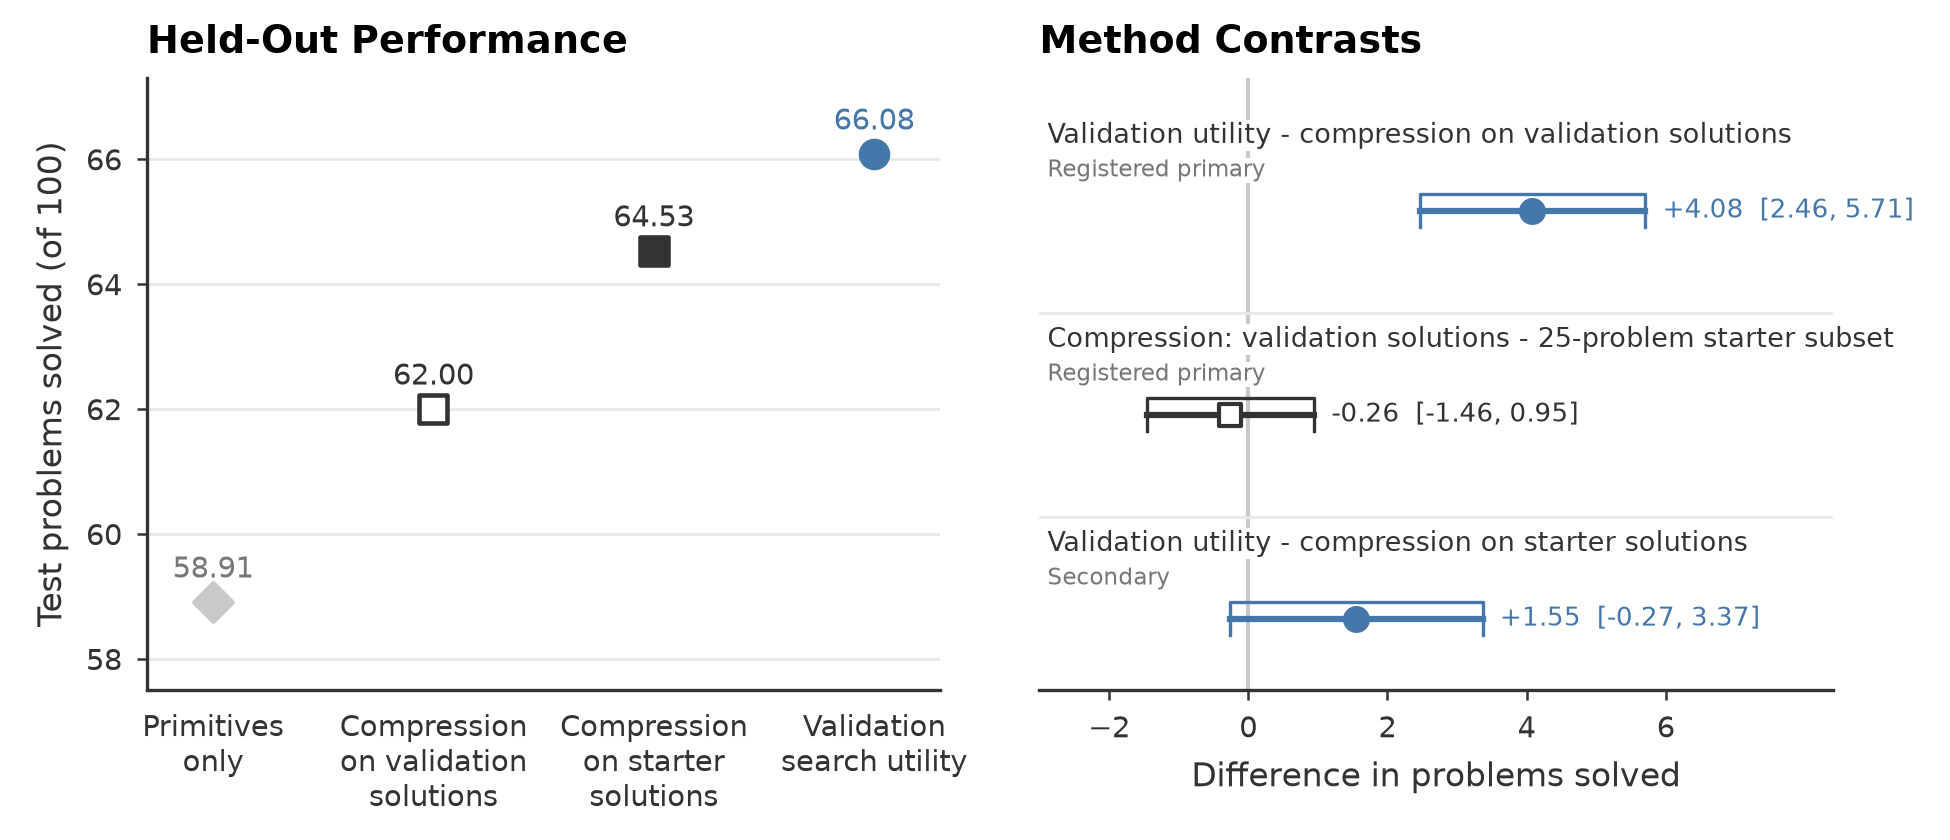
\includegraphics[width=\linewidth]{study_1_selection.png}
  \caption{Experiment I held-out results with ten abstractions. The left graph shows
  means. The right graph shows paired differences with 95\% Student $t$
  intervals for 30 seeds. Both procedures use the same validation problems.
  Utility includes failures; compression omits unsolved targets. The second
  contrast compares validation-solution compression with compression on 25 starter problems.}
  \label{fig:study1-selection}
\end{figure}
Library selection has an initial search cost. A more expensive selection method
is useful only if later search savings recover that initial cost. Utility has a
higher initial search cost than compression because it runs the solver on every
validation target for each trial library. Selected abstractions can later save
search because the solver can reuse stored grids instead of rebuilding them
from primitive operations. We therefore estimate how many future problems are
needed for these savings to recover Utility's higher initial search cost. We
call this the break-even point. The median break-even point was several thousand
future problems. Some seed-condition cases never recovered Utility's higher
initial search cost. Figure~\ref{fig:study1-cost} gives the exact selection
costs, median break-even points, and case counts.
\FloatBarrier
\begin{figure}[!htbp]
  \centering
  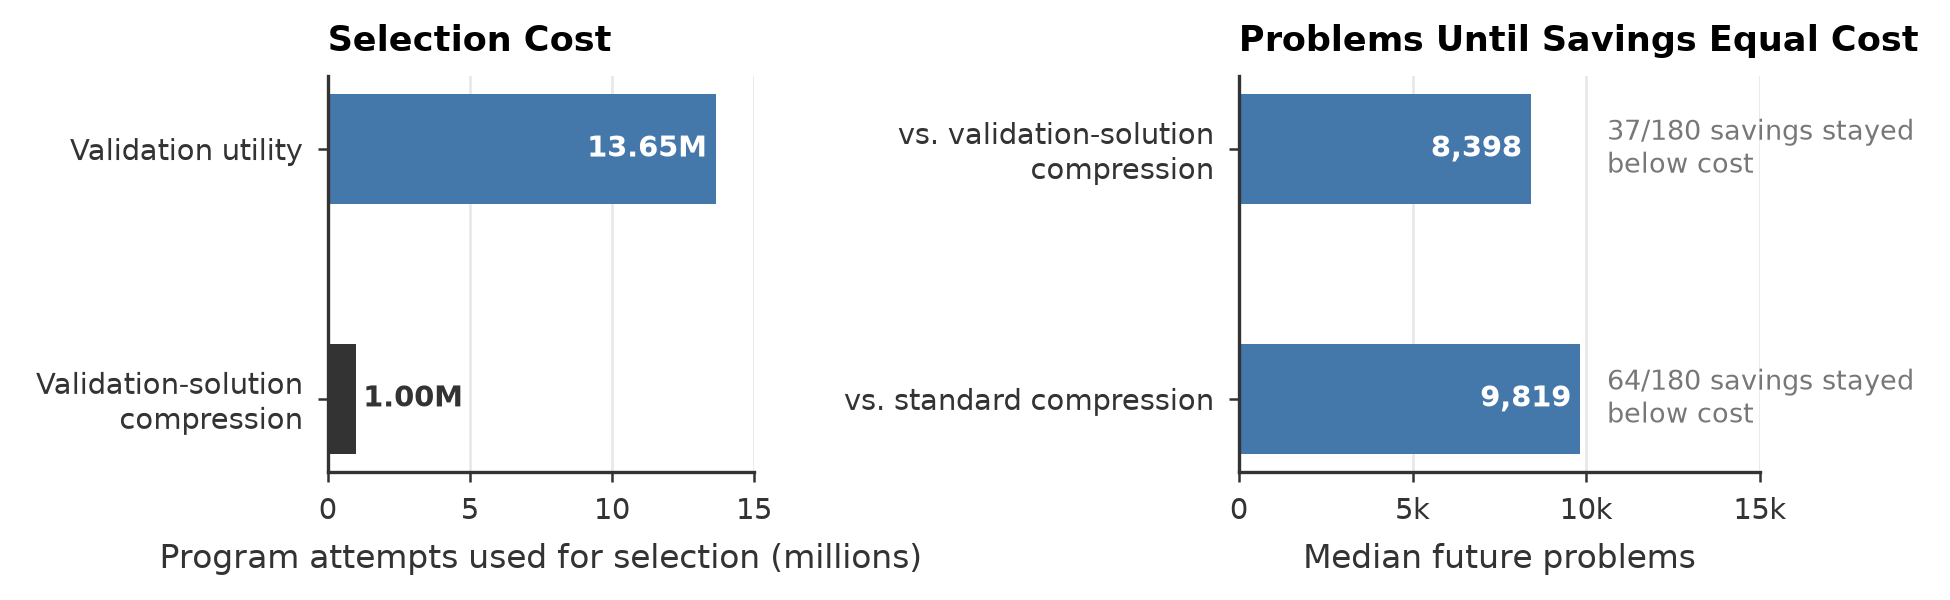
\includegraphics[width=\linewidth]{study_1_cost.png}
  \caption{Selection cost and break-even estimates. Gray labels mark cases
  with no break-even point. Counts omit standard-compression acquisition,
  wall-clock time, and segmentation.}
  \label{fig:study1-cost}
\end{figure}
\FloatBarrier
We expected compression to benefit from similar motifs in starter and test
problems. As hypothesized, utility minus standard compression decreased as
problem-set similarity increased. The mean difference was 2.7 problems for
different sets, 1.5 for moderately similar sets, and 0.5 for similar sets (left
graph in Figure~\ref{fig:study1-secondary}). Assigned shift changed utility
minus validation-solution compression by 1.70 problems (95\% CI [$-0.56$, 3.96]). The
seed-controlled estimate for problem-set similarity was $-0.36$ (95\% CI [$-2.43$, 1.71]); the
slope versus standard compression was $-1.44$ (95\% CI [$-3.18$, 0.30]). The
different-set interval excluded zero, showing utility's advantage in that
group. Formal comparisons across problem-set similarity levels included zero
and did not establish the hypothesized effect.
We also tested whether abstractions chosen via search utility also indirectly compressed solutions. We applied each library post hoc to the same
starter solutions (right graph in Figure~\ref{fig:study1-secondary}). Direct
compression on 25 starter problems removed 25.78\% of operations; utility on
those problems removed 12.32\%; validation utility on 25 validation targets
removed 9.79\%. Utility shortened solutions indirectly. Direct compression
removed more.
\FloatBarrier
\begin{figure}[!htbp]
  \centering
  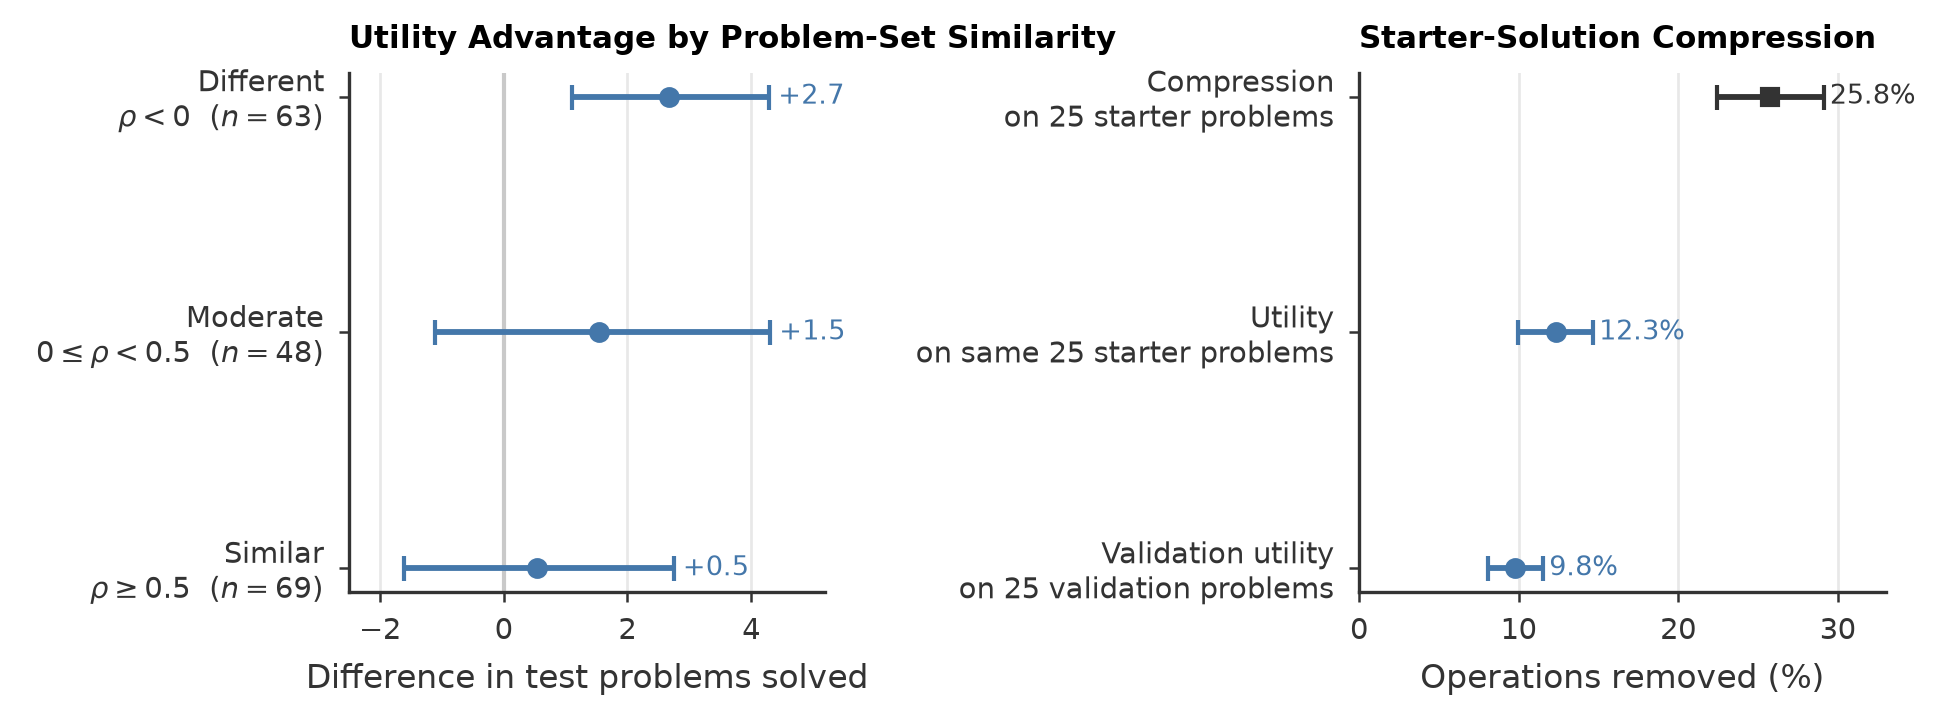
\includegraphics[width=\linewidth]{study_1_secondary.png}
  \caption{Problem-set similarity and indirect compression. Left: utility minus
  standard compression at three problem-set similarity levels. Right: post hoc
  operations removed from the same starter solutions. Intervals are 95\%
  seed-cluster and seed bootstrap, respectively; problem-set similarity bands
  were not registered.}
  \label{fig:study1-secondary}
\end{figure}
\subsection{Experiment II: Library Size}

Held-out performance did not change steadily as library size increased
(Figure~\ref{fig:capacity-budget}). From ten to twenty abstractions, standard
compression lost 12.35 problems (simultaneous 95\% CI [$-13.89$, $-10.81$]),
and utility lost 12.11 (simultaneous 95\% CI [$-13.20$, $-11.02$]). At twenty
abstractions, both libraries solved fewer problems than the primitive-only
library. Utility exceeded
validation-solution compression by 5.13
problems (simultaneous 95\% CI [3.45, 6.80]) and standard compression by 1.73
(simultaneous 95\% CI [$-0.17$, 3.63]). The utility advantage over validation-solution
compression increased by 1.85 from ten to twenty (simultaneous 95\% CI
[$-0.03$, 3.73]). Thus, library size had a larger effect on absolute performance
than on method differences.
At $B=30{,}000$, the descriptive means were highest at $K=11$: 66.32 for
standard compression and 67.85 for utility. From $K=1$ to $K=2$, standard
compression lost 8.08 problems, and utility lost 6.14. For standard
compression, operations removed from starter solutions increased from 24.14\%
at $K=11$ to 27.21\% at $K=20$. Held-out performance decreased over the same
range. Thus, more compression did not ensure better bounded search. This result
motivated Experiment III.
\subsection{Experiment III: Search Budget}

\begin{figure}[!t]
  \centering
  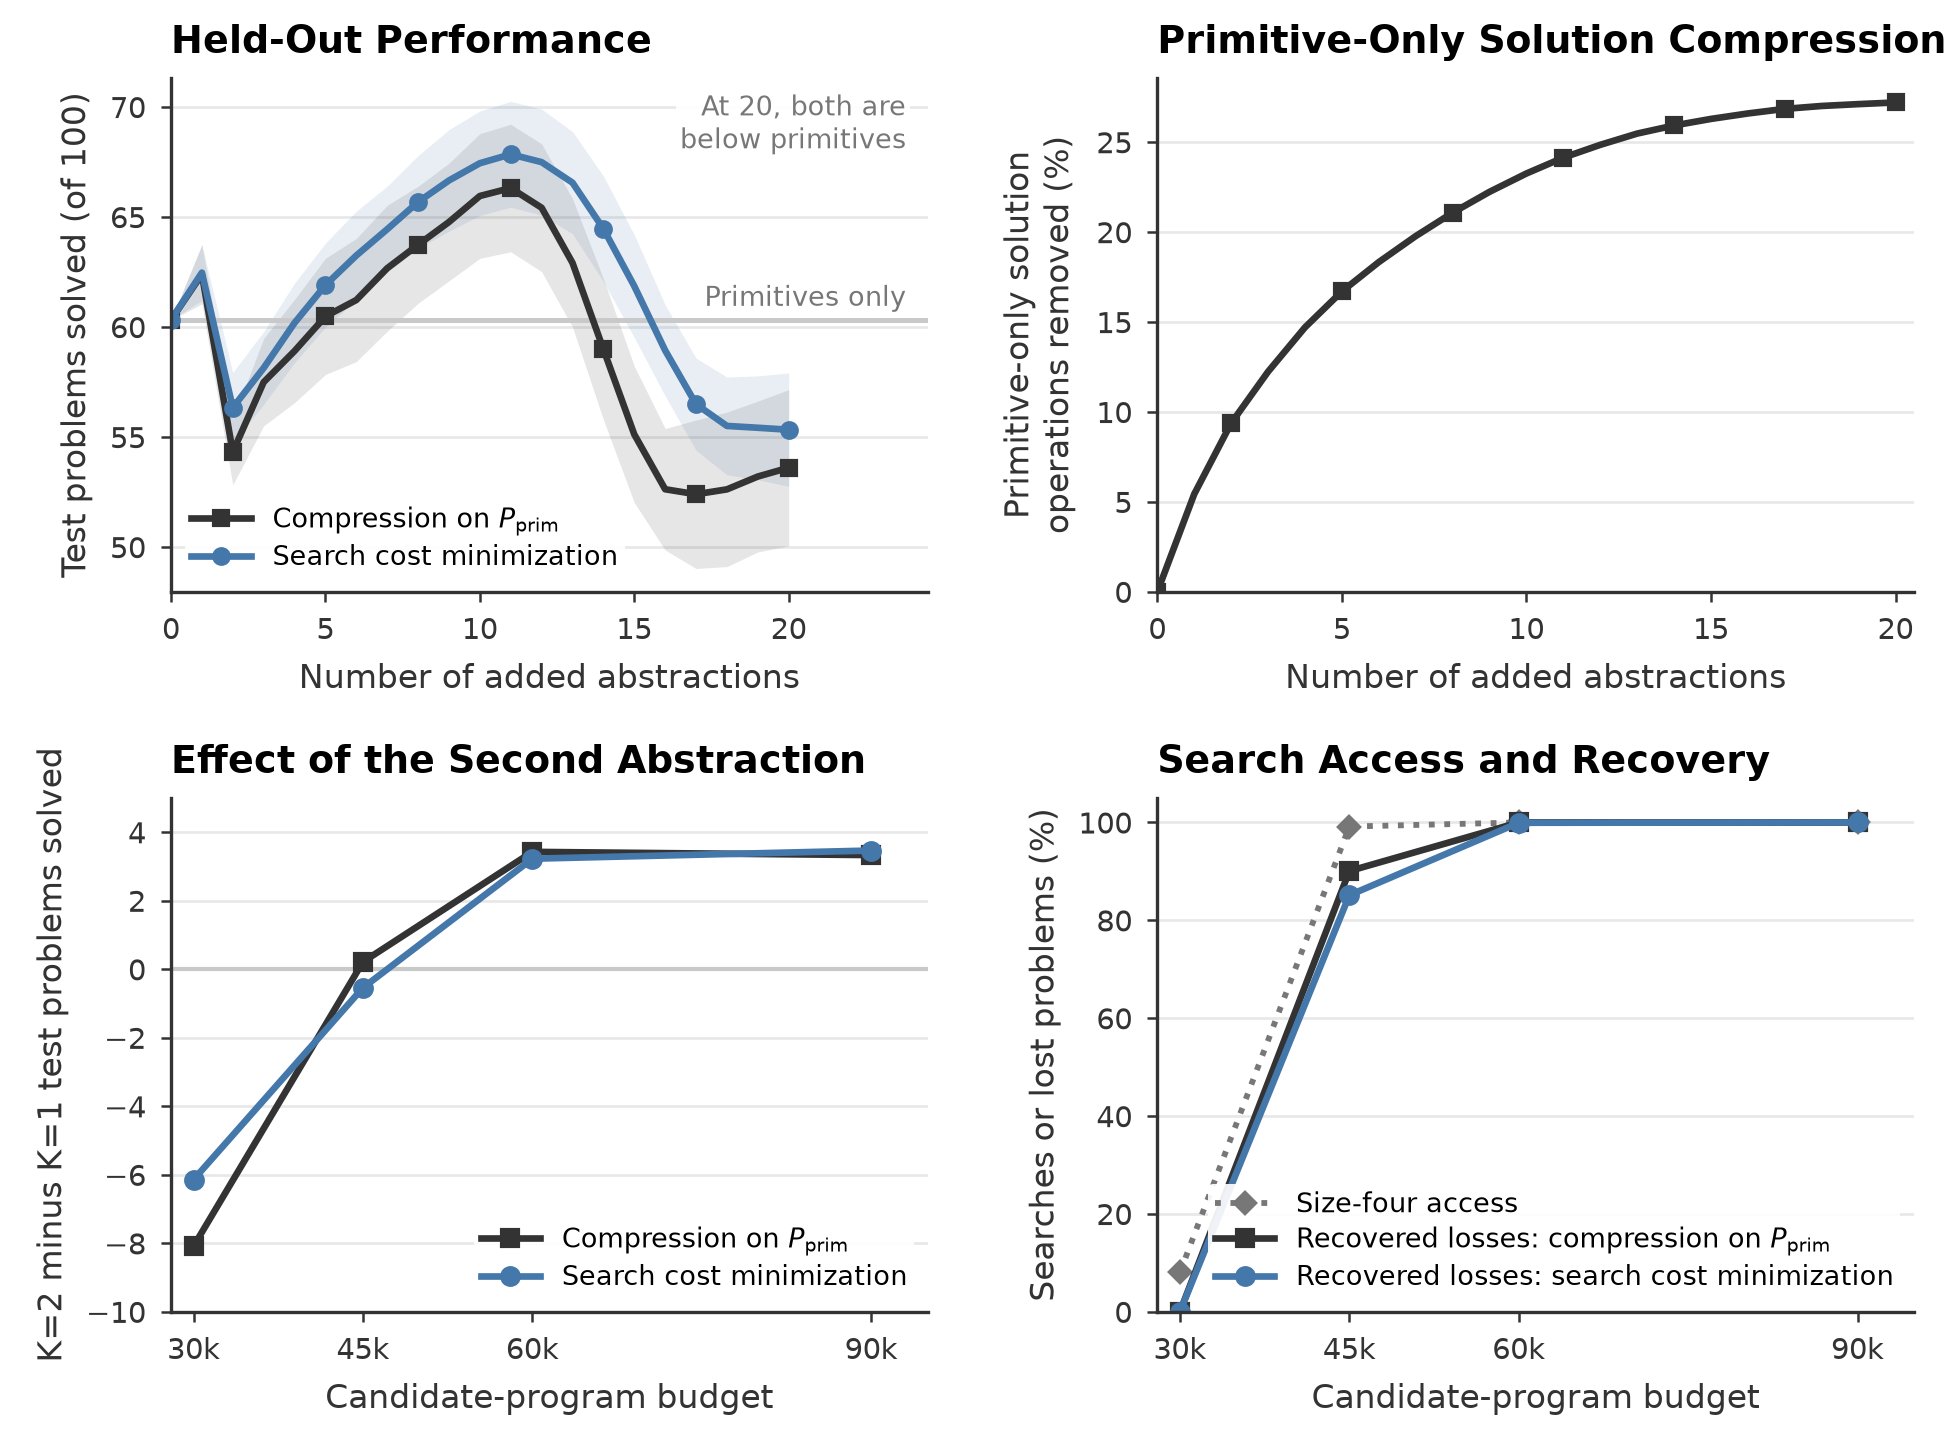
\includegraphics[width=\linewidth]{study_2_3_capacity_budget.png}
  \caption{Experiments II and III. The top row shows held-out performance and
  starter-solution compression across library sizes. The held-out bands are
  simultaneous 95\% intervals. The compression graph is post hoc. At $K=0$,
  the library has only primitives. The bottom row shows the fixed-library
  budget test, size-four access, and descriptive recovery of losses.}
  \label{fig:capacity-budget}
\end{figure}
An increased budget reversed the one-to-two decrease for the fixed libraries
(Figure~\ref{fig:capacity-budget}). As the budget increased from 30,000 to
90,000 program attempts, the second-abstraction effect increased by 11.42
solved problems for standard compression. Its simultaneous 95\% CI was [10.17,
12.66]. The effect increased by 9.61 problems for validation utility. Its
interval was [8.52, 10.69]. At
$B=90{,}000$, the effects were 3.33 for standard compression and 3.47 for
validation utility. All seed-level interactions were positive. With two
abstractions, the share of enumerations that reached size-four programs
increased from 8.1\% at 30,000 attempts to 99.2\% at 45,000 and 100\% at 60,000.
By $B=90{,}000$, the solver recovered all test instances that the
two-abstraction library lost relative to the one-abstraction library at
$B=30{,}000$. Only the budget changed. Thus, the 30,000-attempt budget caused
the one-to-two decrease for these fixed libraries. This result does not set a
sufficient budget for other libraries, solvers, or benchmarks.

\FloatBarrier

\section{Discussion}

The central conclusion is that an abstraction has no fixed value. Its value
depends on selection evidence and objective, library contents, future problems,
solver, search budget, selection cost, and expected reuse.
Experiment I compares the complete selection procedures. Validation utility minimized capped search
cost for all 25 validation targets, including failures. Validation-solution
compression minimized operations in acquired solutions for the same targets
but omitted unsolved targets. With ten abstractions, utility solved 4.08 more held-out
test problems than validation-solution compression. This supports the
hypothesis that complete validation utility selects more useful abstractions
than validation-solution compression. Utility measures bounded search cost,
including added programs and full-budget failures. Compression measures
shortcuts only in acquired solutions. Utility can thus favor lower net search
cost. However, the 4.08-problem difference also reflects solution availability,
so it does not isolate the scoring objective. Utility's
1.55-problem advantage over standard compression remained uncertain. Standard
compression used 100 starter problems, four times as many.
Broader evidence could
explain the smaller difference, but this experiment did not test that
explanation.

How well selection problems match future problems could also change abstraction
value. We therefore hypothesized that compression would become more
competitive as starter and test motif frequencies became more similar. The
means followed this pattern: utility's advantage over standard compression fell
from 2.7 problems for different sets to 0.5 for similar sets. However, the
formal intervals included zero, so the statistical evidence remains
inconclusive. This direction follows because compression rewards stored grids
that replace subtrees in starter solutions.
Recurring motifs can let those grids shorten test solutions. Our problem-set
similarity measure, however, ranks only motif counts and omits operator context,
exact grid reuse, program position, and search order. Similar motif counts do
not ensure similar search value.

Experiment II showed that abstraction value depends on library size. At 30,000
attempts, observed mean performance was highest at 11
abstractions and fell below the primitive-only library at 20. Standard
compression removed more operations from starter solutions as its library grew
from 11 to 20 abstractions, even as held-out performance decreased. Each
abstraction is a size-zero item. Combining it with operators and other library
items creates new low-operation programs. The solver examines them first, so
they can use the budget before it reaches a larger program where the
abstraction helps. A new
item also changes when the solver reaches programs that use earlier items.
Thus, operation removal measures a shortcut within known solutions. It does not
measure the search required to reach those solutions.

Search budget can determine whether this added search prevents a solution or
only delays it. Experiment III changed only the budget for fixed one- and
two-abstraction libraries. The larger budget reversed the one-to-two loss for
both procedures. This supports the budget hypothesis for those libraries. The
share of enumerations that reached size-four programs rose from 8.1\% at 30,000
attempts to 99.2\% at 45,000. This diagnostic gives descriptive support for the
search-cutoff explanation. However, the experiment does not define a sufficient
budget for other library sizes, solvers, or tasks.

Selection cost creates a separate tradeoff because future savings must recover
the initial cost. Validation utility required a bounded search for every trial
library. Among cases with a break-even point, the median required thousands of
future problems. Some experimental cases never reached that point.
Existing representative solutions reduce compression's initial selection cost.
The break-even calculation counts only program attempts, so it does not
estimate total deployment cost.

\section{Limitations and Future Work}

The controls make changes in bounded search easier to identify, but they limit
where the results can apply. This study tests one synthetic, target-only grid
benchmark. Every abstraction is a fixed output grid with size zero. The
primitives, operators, program-size limit, and target generator stay fixed.
Learned functions and parameterized abstractions can apply across inputs and
produce different search costs. Future work should repeat these experiments on
input--output synthesis tasks and in other domains.
A direct comparison of stored grids and learned functions should hold the
solver and budget fixed.

The search-cutoff explanation also depends on the solver. This solver performs
deterministic bottom-up enumeration and orders programs by operation count.
Library order and duplicate removal affect when the solver reaches a target. A
guided solver could prune low-value combinations or reach useful larger
programs sooner. Future studies should compare deterministic enumeration with
guided search and test other costs for abstraction use. A joint sweep can test
whether library size and test performance have the same relation under other
budgets.

Candidate discovery also limits the conclusions. All methods select from the
same 50 starter-derived grids. Validation utility cannot select an abstraction
outside this menu. The menu favors grids
that support at least two starter targets and first appear in programs with one
to four operations. Experiment II evaluates prefixes of one greedy sequence
rather than optimizing each library size. Future work should vary menu
construction and compare greedy selection with joint selection of library items
and their order. A selection objective could also charge for the new programs
that each candidate adds.

The primary Experiment I comparison evaluates complete procedures, so it does
not isolate the scoring objective. Utility scored all 25 validation targets and
failures; compression scored only acquired solutions. The 4.08-problem gap
therefore includes the scoring objective and
solution availability. Standard compression used solutions acquired from 100
starter problems, so its evidence also differed. A same-evidence comparison
should use fixed target-solution pairs. Utility would score the targets, and
compression would score their solutions. Solution acquisition must be fixed
before data collection. The similarity measure has a separate limit: it
requires hidden motif counts from completed test data, so it cannot guide
deployment. Future work should define the measure before data collection and
vary compositional structure directly. More
independent seeds would improve precision.

Several findings need independent confirmation. The observed performance peak
near 11 abstractions and the one-to-two decrease were descriptive.
Experiment III reused the Experiment II seeds and fixed one- and
two-abstraction libraries. Its budget effect applies only to those libraries
and is not an independent replication. An independent test should use new seeds
and libraries. A broader sweep can identify the budgets needed to reach
programs that use added abstractions.

Finally, the break-even analysis counts only program attempts. It omits
wall-clock time, memory use, and compression segmentation. The
standard-compression comparison treats prior starter-solution acquisition as
sunk. The calculation assumes constant mean savings across future problems.
Future work should measure end-to-end acquisition, selection, and evaluation
costs for expected workloads under distribution change.

\newpage
\section{Conclusion}

An abstraction has no fixed value. Its value depends on the data and score used
for selection, the future problems, the library, and the solver. With ten
abstractions, validation utility solved 4.08 more test problems than
validation-solution compression. This difference compares complete procedures
and includes the scoring objective and solution availability. Utility's
advantage over standard compression remained uncertain. Mean performance
differences across problem-set similarity levels followed the hypothesis.
Formal intervals for these differences included zero.

Library size also changed whether selected abstractions helped. At 30,000
attempts, both procedures improved on primitive-only search with ten
abstractions. Mean performance peaked near 11 and fell below primitives alone at
20. Standard compression removed more operations from starter solutions over
this range. Held-out performance decreased. Solution compression alone was an
incomplete measure of bounded-search value. Each added item made more
low-operation programs available. The solver examined these before later
programs where the item could help.

For the fixed libraries, search budget determined whether the solver reached
those later programs. Increasing only the budget reversed the one-to-two loss.
This result supports the search-cutoff explanation for those libraries.
Utility's added selection work often required thousands of future problems to
recover and did not recover in some cells. A practical system should evaluate
the complete library with its intended solver, budget, workload, and expected
reuse. A useful abstraction must save more search than its selection and added
programs cost on that workload.

\section*{Code and Data Availability}

The public repository contains the code, generated data, and reproduction
instructions.
\par\smallskip
\noindent
\href{https://github.com/cucupac/program-synthesis}{%
\mbox{\texttt{github.com/cucupac/program-synthesis}}}.

\bibliography{references_rlj2026}
\bibliographystyle{rlj}

\end{document}
